%!TEX root = ../sample.tex

\section{The POPP Extensions}
\label{sec:popp_extensions}

In~\cite{jovan18a} we demonstrated that the POPP model is able to efficiently correct miscounts made by multiple unreliable counting devices observing a single Poisson process. However, the POPP model is limited by two assumptions:
\begin{enumerate}
	\item the sensors are conditionally independent given the true count, and 
	\item the degree of the unreliability of a sensor (i.e. $\tau$ and $\xi$) is precisely known.
\end{enumerate}
In this paper, we propose three extensions to the POPP model to tackle these assumptions. The first extension (POPP-Beta) extends the POPP model with an observation model which captures uncertainty about the role of the sensor reliability. The second extension (C-POPP) modifies the POPP model to accommodate correlations between sensors. The third extension (POPP-Dirichlet) combines these ideas to jointly address both assumptions. 

\subsection{POPP-Beta}
\label{subsec:popb}

The POPP model requires the true positive and false positive rates to be specified for sensor $j$, i.e.  $\tau_j = P_j(d \mid e{=}1)$ and $\xi_j = P_j(d \mid e{=}0)$. 
The POPP model requires these rates to be accurate in order to generate correct posteriors over $\lambda$. To accurately determine the rates in practice, one needs to have a large data set of both sensed counts and the ground truth. Given the ground truth is typically manually created, this places a large burden on experts who need to label the data.   

Here, we extend the original POPP model to take into account uncertainty in the true and false positive rates due to limited training data.
% 
To model this uncertainty we use Bayesian estimation to determine the 
true positive rate ($\tau$) and false positive rate ($\xi$).
% 
We use Beta distributions as priors for $\tau$ and $\xi$ because the Beta distribution act as a conjugate to the binomial distribution, providing a family of prior probability distributions for the parameter of a binomial distribution. The Beta-binomial conjugacy leads to an analytically tractable compound distribution called the Beta-binomial distribution $BB(d \mid c, \zeta, \eta)$, where the $p$ parameter in the binomial distribution $B(d \mid c, p)$ is drawn from a Beta distribution $Be(p \mid \zeta, \eta)$.

\begin{figure}[t!]
	\centering
	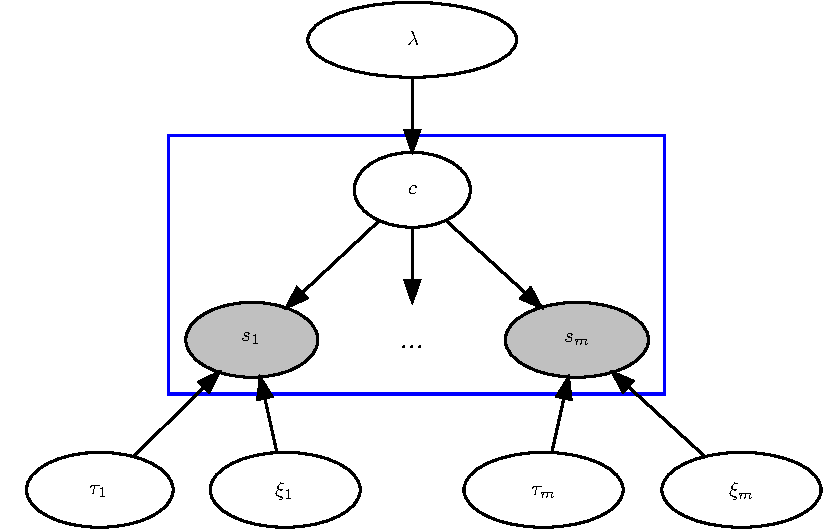
\includegraphics[width=0.75\textwidth]{./figures/popb-pics.pdf}
	\caption{Graphical representation of the POPP-Beta. Instead of having fixed estimated points for the sensor rates $\tau$ and $\xi$ like in the POPP model, they are represented by Beta distributions in the POPP-Beta.}
	\label{fig:gm_popb}
	\vspace{-20pt}
\end{figure}

% \begin{equation}
% 	\label{eq:beta_binomial}
% 	\begin{tabular}{r@{ = }l}
% 		$P(d ; c, \zeta, \eta)$ & $\displaystyle\int_{0}^{1} P(d ; c, p) ~ P(p ; \zeta, \eta) ~dp$ \\ [2ex]
% 		& $\displaystyle\int_{0}^{1} B(d ; c, p) ~ Be(p ; \zeta, \eta) ~dp$ \\ [2ex]
%         & $\displaystyle\int_{0}^{1} \binom{c}{d} p^d (1-p)^{(c-d)} ~ \displaystyle\frac{p^{(\zeta - 1)} (1-p)^{(\eta-1)}}{\pi(\zeta, \eta)}$ \\ [2ex]
%         & $\displaystyle\binom cd \displaystyle\frac{1}{\pi(\zeta, \eta)} \displaystyle\int_{0}^{1} p^{(d+\zeta-1)} (1-p)^{(c-d+\eta-1)} dp$ \\ [2ex]
%         & $\displaystyle\binom cd \displaystyle\frac{\pi(d+\zeta, c-d+\eta)}{\pi(\zeta, \eta)}$ \\ [2ex]
%         & $BB(d ; c, \zeta, \eta)$
% 	\end{tabular}
% \end{equation}

Our sensor rates, $\tau_j$ and $\xi_j$, are now estimated from two Beta distributions: $Be(\tau \mid \zeta_{\tau}, \eta_{\tau})$ and $Be(\xi \mid \zeta_{\xi}, \eta_{\xi})$.
% 
$\zeta_{\tau}$ and $\zeta_{\xi}$ are the number of true positive and false positive detections in the ground truth data respectively.
% 
$\eta_{\tau}$ and $\eta_{\xi}$ are the number of true negative and false  negative detections in the ground truth data respectively. 
% 
Given these parameters, we form the POPP-Beta model from POPP by replacing Eq. \ref{eq:joint_binomial_distribution} with:  

\begin{equation}
	\label{eq:joint_beta_binomial_distribution}
    P(s_{j,i} \mid c_i) \! = \! \! \! \displaystyle\sum_{r = 0}^{c_{i}} \! \! ~ BB\Big(r \Bigm| c_i, \zeta_{\tau}, \eta_{\tau} \Big) BB\Big( \delta_s r \Bigm| \delta_c r, \zeta_{\xi}, \eta_{\xi} \Big)
\end{equation}

\noindent with $\delta_s r = (s_{j,i} - r)$, and $\delta_c r = (l - c_i)$.

% With a sensor model which follows beta densities and is fully integrated, as a distribution, in the sensed count likelihood $P(s_{ji} ; c_i)$ as shown in Equation \ref{eq:joint_beta_binomial_distribution}, we obtain a graphical model with the structure shown in Figure \ref{fig:gm_popp_beta}.
One should note that the difference between the POPP and POPP-Beta model, lies only in the change from Eq. \ref{eq:joint_binomial_distribution} to \ref{eq:joint_beta_binomial_distribution}. However, given little training data for the observation model, the POPP-Beta model is expected to be more conservative in estimating the posterior $P(\lambda \mid \mathbf{s})$ over $\lambda$ than the POPP model. 

% \begin{figure*}[t!]
% 	\centering
% 	\begin{tikzpicture}
% 	\tikzstyle{place}=[rectangle,draw=blue,thick,minimum size=5 mm]
% 	\tikzstyle{empty}=[rectangle,draw=white,thick,minimum size=5 mm]
% 	\tikzstyle{every label}=[black]
% 	\begin{scope}
% 	\node[place](31)[xshift=0mm]{$S_{1i}$};
% 	\node[place](32)[right of=31, xshift=20mm]{$S_{2i}$};
% 	\node[place](33)[right of=32, xshift=20mm]{$\ldots$};
% 	\node[place](34)[right of=33, xshift=20mm]{$S_{(m-1)i}$};
% 	\node[place](35)[right of=34, xshift=22mm]{$S_{mi}$};
% 	\node[place](21)[above of=33]{$X_i$} edge[post](31) edge[post](32) edge[post](33) edge[post](34) edge[post](35);
% 	\node[place](11)[above of=21]{$\lambda$} edge[post](21);
%     \node[place](12)[right of=11, xshift=20mm]{$\textrm{tpr}_{(m-1)}, \textrm{xi}_{(m-1)}$} edge[post](34);
%     \node[place](13)[left of=11, xshift=-20mm]{$\textrm{tpr}_{2}, \textrm{xi}_{2}$} edge[post](32);
%     \node[place](14)[right of=12, xshift=22mm]{$\textrm{tpr}_{m}, \textrm{xi}_{m}$} edge[post](35);
%     \node[place](15)[left of=13, xshift=-20mm]{$\textrm{tpr}_{1}, \textrm{xi}_{1}$} edge[post](31);
% 	\node[empty](01)[above of=11]{};
%     \node[place](02)[above of=12]{$(\zeta, \eta)_{\textrm{tpr}}, (\zeta, \eta)_{\textrm{xi}}$} edge[post](12);
%     \node[place](03)[above of=13]{$(\zeta, \eta)_{\textrm{tpr}}, (\zeta, \eta)_{\textrm{xi}}$} edge[post](13);
%     \node[place](04)[above of=14]{$(\zeta, \eta)_{\textrm{tpr}}, (\zeta, \eta)_{\textrm{xi}}$} edge[post](14);
%     \node[place](05)[above of=15]{$(\zeta, \eta)_{\textrm{tpr}}, (\zeta, \eta)_{\textrm{xi}}$} edge[post](15);
% 	\end{scope}
% 	\end{tikzpicture}
%     \caption{Graphical representation of the POPP-Beta.}
% 	\label{fig:gm_popp_beta}
% \end{figure*}